\documentclass{article}
\usepackage{graphicx}
\usepackage{amsmath}
\usepackage{amssymb}
\usepackage[a4paper, top=25mm, bottom=25mm, left=25mm, right=25mm]{geometry}
\usepackage{pgfplots}
\pgfplotsset{compat=1.18}
\usepackage{mathtools}

\begin{document}
\pagestyle{empty}
\large

\begin{center}
2022-2023 Spring \\MAT124 Midterm\\(08/05/2023)
\end{center}

\noindent 1. Sketch the traces of the following surfaces with the coordinate planes $x=0,\:y=0$, and $z=0$, and then sketch the graphs of them.

\hfill

\noindent (a) $\displaystyle\frac{x^2}{16}+\frac{y^2}4-z^2=1$

\hfill

\noindent (b) $\displaystyle z=\frac{x^2}4+\frac{y^2}4-6$

\hfill

\noindent 2. Show that the limit

\[\lim_{(x,y)\to(0,0)}\frac{y^3\sqrt x}{2\left(x^2+y^4\right)}\]

\hfill

\noindent does not exist.

\hfill

\noindent 3. Find the equation of the plane passing through the point $P_0(0,1,2)$ and which is perpendicular to the line that is tangent to the curve of intersection of the surfaces

\[xz^2-2xy+y^2=2\qquad\text{and}\qquad xz-x^2y+z^2=1\]

\hfill

\noindent at the point $P_1\left(0,\sqrt2, 1\right)$.

\hfill

\noindent 4. Find $\displaystyle\frac{\partial w}{\partial s}$ where $w=xy\ln\left(1+\sqrt{x^2+y^2}\right)+xz$ and $x=t+s,\:y=\mathrm{e}^s,\:z=\ln\left(s^2+t\right)$.

\hfill

\noindent 5. Use incremental approximation to estimate the value $\tan\left((0.97)\cdot(2.05)^2\right)$.

\hfill

\noindent 6. Find the direction vector in which the function

\[f(x,y,z)=\sqrt{x+yz}\]

\hfill

\noindent has the minimum rate of change at the point $(1,1,3)$. Also, find this rate of change.

\hfill


\noindent 7. Find the absolute extrema of

\[f(x,y)=x^2+y-xy+4\]

\hfill

\noindent on the triangular region with vertices $(0,0),\:(4,0),\:(0,4)$.

\newpage

\begin{center}
2022-2023 Spring Midterm (08/05/2023) Solutions\\
(Last update: 8/25/25 (25th of August) 11:50 PM)
\end{center}

\noindent 1.

\hfill

\noindent (a)
\begin{center}
\begin{tikzpicture}
  \begin{axis}[
  title={Plane $x=0$},
    xlabel=$y$, ylabel=$z$,
    xtick=\empty, ytick=\empty,
    samples=50,
    axis lines=middle,
    clip=true,
    scale=1,
    enlargelimits=true
    ]
    \addplot[domain=-5:-2, blue] {sqrt(x^2/4-1)};
    \addplot[domain=2:5, blue] {sqrt(x^2/4-1)};
    \addplot[domain=-5:-2, blue] {-sqrt(x^2/4-1)};
    \addplot[domain=2:5, blue] {-sqrt(x^2/4-1)};

    \node[blue] at (2.1,-2) {$\dfrac{y^2}4-z^2=1$};
  \end{axis}
\end{tikzpicture}\hspace{1em}
\begin{tikzpicture}
  \begin{axis}[
  title={Plane $y=0$},
    xlabel=$x$, ylabel=$z$,
    xtick=\empty, ytick=\empty,
    samples=50,
    axis lines=middle,
    clip=true,
    scale=1,
    enlargelimits=true
    ]
    \addplot[domain=-8:-4, red] {sqrt(x^2/16-1)};
    \addplot[domain=4:8, red] {sqrt(x^2/16-1)};
    \addplot[domain=-8:-4, red] {-sqrt(x^2/16-1)};
    \addplot[domain=4:8, red] {-sqrt(x^2/16-1)};

    \node[red] at (3.5,-1.5) {$\dfrac{x^2}{16}-z^2=1$};
  \end{axis}
\end{tikzpicture}

\hfill

\begin{tikzpicture}
  \begin{axis}[
  title={Plane $z=0$},
  axis equal image,
    xlabel=$x$, ylabel=$y$,
    xtick=\empty, ytick=\empty,
    samples=200,
    axis lines=middle,
    clip=true,
    scale=1,
    enlargelimits=true
    ]
    \addplot[domain=-4:4, orange] {4*sqrt(1-x^2/16)};
    \addplot[domain=-4:4, orange] {-4*sqrt(1-x^2/16)};

    \node[orange] at (1.9,1.1) {\small $\dfrac{x^2}{16}+\dfrac{y^2}4=1$};
  \end{axis}
\end{tikzpicture}\hspace{1em}
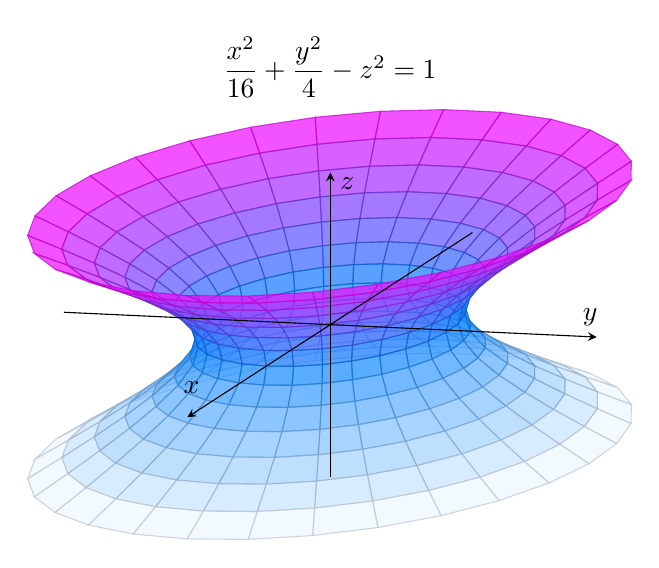
\begin{tikzpicture}
  \begin{axis}[
    title={$\dfrac{x^2}{16}+\dfrac{y^2}4-z^2=1$},
    title style={yshift=-20pt},
      view={105}{10},
      axis lines=center,
      axis equal image,
      xlabel={$x$},
      ylabel={$y$},
      zlabel={$z$},
      domain=0:2*pi,
      y domain=-2:2,
      samples=30,
      samples y=15,
      zmin=-2.5, zmax=2.5,
      colormap/cool,
      axis on top,
      scale=2.5,
      xtick=\empty, ytick=\empty, ztick=\empty,
      z buffer=sort,
    ]
    \addplot3[
      surf,
      opacity=0.7
    ]
    ( {4*sqrt(1+y^2)*cos(deg(x))},
      {2*sqrt(1+y^2)*sin(deg(x))},
      {y} );
  \end{axis}
\end{tikzpicture}
\end{center}

\hfill

\noindent (b)
\begin{center}
\begin{tikzpicture}
  \begin{axis}[
  title={Plane $x=0$},
    xlabel=$y$, ylabel=$z$,
    xtick=\empty, ytick=\empty,
    samples=50,
    axis lines=middle,
    clip=true,
    scale=1,
    enlargelimits=true
    ]
    \addplot[domain=-5:5, blue] {x^2/4-6};

    \node[blue] at (1.9,-1.8) {$z=\dfrac{y^2}4-6$};
  \end{axis}
\end{tikzpicture}\hspace{1em}
\begin{tikzpicture}
  \begin{axis}[
  title={Plane $y=0$},
    xlabel=$x$, ylabel=$z$,
    xtick=\empty, ytick=\empty,
    samples=50,
    axis lines=middle,
    clip=true,
    scale=1,
    enlargelimits=true
    ]
    \addplot[domain=-5:5, red] {x^2/4-6};

    \node[red] at (1.9,-1.8) {$z=\dfrac{x^2}4-6$};
  \end{axis}
\end{tikzpicture}

\begin{tikzpicture}
  \begin{axis}[
  title={Plane $z=0$},
  axis equal image,
    xlabel=$x$, ylabel=$y$,
    xtick=\empty, ytick=\empty,
    samples=300,
    axis lines=middle,
    clip=true,
    scale=1,
    enlargelimits=true
    ]
    \addplot[domain=-2*sqrt(6):2*sqrt(6), orange] {sqrt(24-x^2)};
    \addplot[domain=-2*sqrt(6):2*sqrt(6), orange] {-sqrt(24-x^2)};

    \node[orange] at (2.4,0.8) {\small $y^2=24-x^2$};
  \end{axis}
\end{tikzpicture}\hspace{1em}
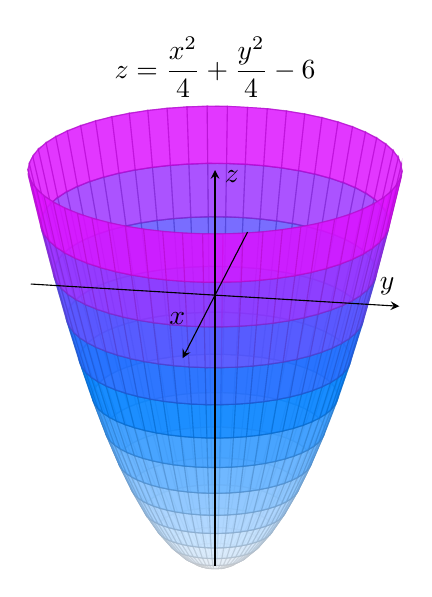
\begin{tikzpicture}
  \begin{axis}[
    title={$\displaystyle z=\frac{x^2}4+\frac{y^2}4-6$},
    title style={yshift=-10pt},
      view={100}{20},
      axis lines=center,
      axis equal image,
      xlabel={$x$},
      ylabel={$y$},
      zlabel={$z$},
      domain=0:2*pi,
      y domain=-2.25:2.25,
      samples=30,
      samples y=30,
      colormap/cool,
      axis on top,
      scale=1.5,
      xtick=\empty, ytick=\empty, ztick=\empty,
      z buffer=sort,
    ]
    \addplot3[
      surf,
      opacity=0.6
    ]
    ( {y*cos(deg(x))},
      {y*sin(deg(x))},
      {y^2-2*sqrt(3)} );
  \end{axis}
\end{tikzpicture}
\end{center}

\hfill

\noindent 2. Apply the Two-Path Test.

\[x=y\implies\lim_{(x,y)\to(0,0)}\frac{y^3\sqrt x}{2\left(x^2+y^4\right)}=\lim_{x\to0}\frac{x^{7/2}}{2\left(x^2+x^4\right)}=\lim_{x\to0}\frac{x^{3/2}}{2\left(1+x^2\right)}=\frac02=0\]
\[x=y^2\implies\lim_{(x,y)\to(0,0)}\frac{y^3\sqrt x}{2\left(x^2+y^4\right)}=\lim_{y\to0}\frac{y^4}{4y^4}=\lim_{y\to0}\frac14=\frac14\]

\hfill

\noindent Since $0\neq\dfrac14$, by the Two-Path Test, the limit does not exist.

\hfill

\noindent 3. Let $f(x,y,z)=xz^2-2xy+y^2=2$ and $g(x,y,z)=xz-x^2y+z^2=1$ be the level surfaces. The cross product of the gradient of these functions give us the vector that is parallel to the line of intersection. Compute the gradients.

\[\nabla f=\left\langle z^2-2y,\:-2x+2y,\:2xz\right\rangle,\quad \nabla g=\left\langle z-2xy,\:-x^2,\: x+2z\right\rangle\]
\[\nabla f\,|_{\left(0,\,\sqrt2,\,1\right)}=\left\langle1-2\sqrt2,\:2\sqrt2,\:0\right\rangle,\quad \nabla g\,|_{\left(0,\,\sqrt2,\,1\right)}=\left\langle1,\:0,\:2\right\rangle\]

\hfill

\noindent Find the cross product.

\begin{align*}\mathbf{n}&=\nabla f\times \nabla g=\left|\begin{array}{ccc}
\mathbf{i}&\mathbf{j}&\mathbf{k}\\
1-2\sqrt2&2\sqrt2&0\\
1&0&2
\end{array}\right|\\\\&=\mathbf{i}\left|\begin{array}{cc}
2\sqrt2&0\\0&2
\end{array}\right|-\mathbf{j}\left|\begin{array}{cc}
1-2\sqrt2&0\\1&2
\end{array}\right|+\mathbf{k}\left|\begin{array}{cc}
1-2\sqrt2&2\sqrt2\\1&0
\end{array}\right|\\\\&=\left(2\sqrt2\cdot2-0\cdot0\right)\mathbf{i}-\left[\left(1-2\sqrt2\right)\cdot2-0\cdot1\right]\mathbf{j}+\left[\left(1-2\sqrt2\right)\cdot0-2\sqrt2\cdot1\right)\mathbf{k}\\\\&=4\sqrt2\,\mathbf{i}+\left(4\sqrt2-2\right)\,\mathbf{j}+-2\sqrt2\,\mathbf{k}\end{align*}

\hfill

\noindent The line of intersection is the normal line of the plane. Therefore, $\mathbf n$ is the normal vector of the plane. The equation of the plane with the normal vector $\mathbf n$ and containing the point $P(x_0,y_0,z_0)$ is

\[n_1(x-x_0)+n_2(y-y_0)+n_3(z-z_0)=0\]

\hfill

\noindent Therefore, the equation for this plane is

\[4\sqrt2(x-0)+\left(4\sqrt2-2\right)(y-1)-2\sqrt2(z-2)=0\]

\[\boxed{2x\sqrt2+y\left(2\sqrt2-1\right)-z\sqrt2+1=0}\]

\hfill

\noindent 4. Apply the chain rule.

\[\frac{\partial w}{\partial s}=\frac{\partial w}{\partial x}\cdot\frac{\partial x}{\partial s}+\frac{\partial w}{\partial y}\cdot\frac{\partial y}{\partial s}+\frac{\partial w}{\partial z}\cdot\frac{\partial z}{\partial s}\]

\hfill

\noindent Compute the partial derivatives.

\[\frac{\partial w}{\partial x}=y\ln\left(1+\sqrt{x^2+y^2}\right)+xy\cdot\frac1{1+\sqrt{x^2+y^2}}\cdot\left(\frac{x}{\sqrt{x^2+y^2}}\right)+z\]
\[\frac{\partial w}{\partial y}=x\ln\left(1+\sqrt{x^2+y^2}\right)+xy\cdot\frac1{1+\sqrt{x^2+y^2}}\cdot\left(\frac{y}{\sqrt{x^2+y^2}}\right),\quad \frac{\partial w}{\partial z}=x\]

\[\frac{\partial x}{\partial s}=1,\quad\frac{\partial y}{\partial s}=\mathrm{e}^s,\quad\frac{\partial z}{\partial s}=\frac{2s}{s^2+t}\]

\begin{align*}\frac{\partial w}{\partial s}=&\left[y\ln\left(1+\sqrt{x^2+y^2}\right)+xy\cdot\frac1{1+\sqrt{x^2+y^2}}\cdot\left(\frac{x}{\sqrt{x^2+y^2}}\right)+z\right]\cdot1\\\\&+\left[x\ln\left(1+\sqrt{x^2+y^2}\right)+xy\cdot\frac1{1+\sqrt{x^2+y^2}}\cdot\left(\frac{y}{\sqrt{x^2+y^2}}\right)\right]\cdot\mathrm{e}^s+\frac{2xs}{s^2+t}\end{align*}

\hfill

\noindent Write in terms of $s$ and $t$ rigorously.

\[\boxed{\begin{array}{ll}\dfrac{\partial w}{\partial s}=&
\mathrm{e}^s\ln\left(1+\sqrt{(t+s)^2+\mathrm{e}^{2s}}\right)+\dfrac{(t+s)^2\cdot\mathrm{e}^s}{\sqrt{(t+s)^2+\mathrm{e}^{2s}}+(t+s)^2+\mathrm{e}^{2s}}+\ln\left(s^2+t\right)\\\\&+(t+s)\mathrm{e}^s\ln\left(1+\sqrt{(t+s)^2+\mathrm{e}^{2s}}\right)+\dfrac{(t+s)\cdot\mathrm{e}^{3s}}{\sqrt{(t+s)^2+\mathrm{e}^{2s}}+(t+s)^2+\mathrm{e}^{2s}}\\\\&+\dfrac{2s(t+s)}{s^2+t}
\end{array}}\]

\hfill

\noindent 5. Let $f(x,y)=\tan\left(xy^2\right)$. The total differential of $f$ is

\[df=f_x\,dx+f_y\,dy=\sec^2\left(xy^2\right)\cdot y^2\,dx+\sec^2\left(xy^2\right)\cdot2xy\,dy\]

\hfill

\noindent Since $x=0.97\approx1$ and $y=2.05\approx2$, we may approximate the value of $\tan\left(0.97\cdot2.05^2\right)$ near $\tan\left(1\cdot 2^2\right)=\tan4$. Take $x=1,\:y=2,\:dx=0.97-1=-0.03,\:dy=2.05-2=0.05$.

\[df=\sec^24\cdot4\cdot(-0.03)+\sec^24\cdot4\cdot(0.05)=0.08\sec^24\]

\hfill

\noindent Since $f(x+\Delta x,\:y+\Delta y)\approx f(x,y)+df$, the value of $\tan\left(0.97\cdot2.05^2\right)$ is approximately

\[\boxed{\tan4+0.08\sec^24}\]

\hfill

\noindent 6. The function $f$ has the minimum rate of change if the gradient vector of $f$ and the unit direction vector $\mathbf u$ are antiparallel. That is, they have opposite directions.

\[\nabla f=\left\langle\frac1{2\sqrt{x+yz}},\frac z{2\sqrt{x+yz}},\frac y{2\sqrt{x+yz}}\right\rangle\]

\[\left(\nabla f\cdot \mathbf u\right)_{\text{min}}=\left|\nabla f\right||u|\cos\pi=-|\nabla f|\]

\[\nabla f|_{(1,1,3)}=\left\langle\frac14,\frac34,\frac14\right\rangle\implies-|\nabla f|=-\sqrt{\left(\frac14\right)^2+\left(\frac34\right)^2+\left(\frac14\right)^2}=-\frac{\sqrt{11}}4\]

\hfill

\noindent Since $\mathbf u$ has the opposite direction to that of the gradient, we may also find the components of $\mathbf u$.

\[\mathbf{u}=-\frac{\nabla f}{|\nabla f|}=-\frac{\left\langle\frac14,\frac34,\frac14\right\rangle}{\frac{\sqrt{11}}4}=\left\langle-\frac1{\sqrt{11}},-\frac3{\sqrt{11}},-\frac1{\sqrt{11}}\right\rangle\]

\[\boxed{\text{The minimum rate of change: }{-\frac{\sqrt{11}}4},\text{ the direction vector:}\left\langle-\frac1{\sqrt{11}},-\frac3{\sqrt{11}},-\frac1{\sqrt{11}}\right\rangle}\]

\hfill

\noindent 7. $f$ is continuous on a bounded and closed set on $\mathbb R$. By the Extreme Value Theorem, the extrema must exist in the region or on the boundary.

\hfill

\noindent First, determine where $f_x=f_y=0$ to find the critical points.

\[f_x=2x-y,\quad f_y=1-x\]
\[f_x=f_y=0\implies2x-y=0,\quad1-x=0\implies x=1,\quad y=2\]
\[f(1,2)=5\]

\hfill

\noindent Take a look at the boundary. From $(0,0)$ to $(4,0)$, we have $y=0$.

\[y=0\implies f(x,0)=x^2+4\quad\rightarrow\quad\frac d{dx}\left(x^2-4\right)=2x=0\implies x=0\]
\[f(0,0)=4\]

\hfill

\noindent From $(0,0)$ to $(0,4)$, we have $x=0$.

\[x=0\implies f(0,y)=y+4\quad\rightarrow\quad\frac d{dy}\left(y+4\right)=1\neq0\]

\hfill

\noindent From $(4,0)$ to $(0,4)$, we have $x=y$.

\[y=4-x\implies f(x,4-x)=x^2+(4-x)-x(4-x)+4=2x^2-5x+8\]

\[\frac d{dx}\left(2x^2-5x+8\right)=4x-5=0\implies x=\frac54,\quad y=\frac{11}4\]
\[f\left(\frac54,\frac{11}4\right)=\frac{39}8\]

\hfill

\noindent We also have $f(0,0)=5,\:f(4,0)=20,\:f(0,4)=8$ from the vertices of the triangular region.

\hfill

\noindent Compare all the values $f(0,0),\:f(1,2),\:f(4,0),\:f(0,4),\:f\left(\frac54,\frac{11}4\right)$.

\[\boxed{\text{Absolute minimum: }f(0,0)=4,\quad \text{absolute maximum: } f(4,0)=20.}\]

\end{document}